\chapter{Tests}

\section{TrainTest}

Um den Code für den Raspberry Pi testen zu können wurde die Klasse TrainTest (Abbildung \ref{pic:train_test}) entworfen. Genau wie die eigentliche Implementierung beinhaltet die Testklasse unsere Socketimplementierung zur Kommunikation mit dem Server. Um eine möglichst große Testabdeckung zu erreichen besitzt die Klasse zwei Startthreads, TrainTestThread und TrainTestFailureThread. Zwischen diesen kann durch die Auswahl einer "Initial instance" in den Features einer Component unterschieden werden.

\subsection{TrainTestThread}

Durch das Ausführen des TrainTestThread startet ein Idealer Ablauf des Zuges. Genau wie beim Start des echten Zuges muss auch die Testklasse zuerst einen Tag an den Server übermitteln. Dieser wird zufällig aus einer Liste mit erlaubten Starttags ausgewählt, die die möglichen Bahnhöfe darstellen soll. Über die Socketverbindung ankommende Befehle beinhalten den Tag, an dem eine Geschwindigkeitsänderung erfolgen soll. Da dies der nächste zu erwartende Tag ist wird genau dieser Tag mit einer Verzögerung von 5 Sekunden zurück. Es wird also der perfekte Ablauf des Zuges erwartet.

\subsection{TrainTestFailureThread}

Um auch einen fehlerhaften Ablauf simulieren zu können wurde die Klasse TrainTestFailureThread erstellt. Auch diese Klasse wählt zu beginn einen zufälligen Tag aus einer Liste mit erlaubten Starttags und übermittelt diesen an den Server. Für jeden nun ankommenden Befehl des Servers wird eine Variable inkrementiert und mittels Modulo zwischen drei Möglichkeiten unterschieden:

\begin{enumerate}
	\item Senden des Tags aus dem empfangenen Befehl.
	\item Senden des letzten Tags. Der Zug liest also erneut den letzten Tag, als wäre er im Kreis gefahren. Entspricht auch einem Falsch gelesenen Tag.
	\item Senden des nächsten Tags. Dazu wird der als float gespeicherte Wert des Tags einfach um 0.5 erhöht, was einem übersprungenen Tag entspricht.
\end{enumerate}

\begin{figure}
	\caption{Die Testklasse des Zuges}
	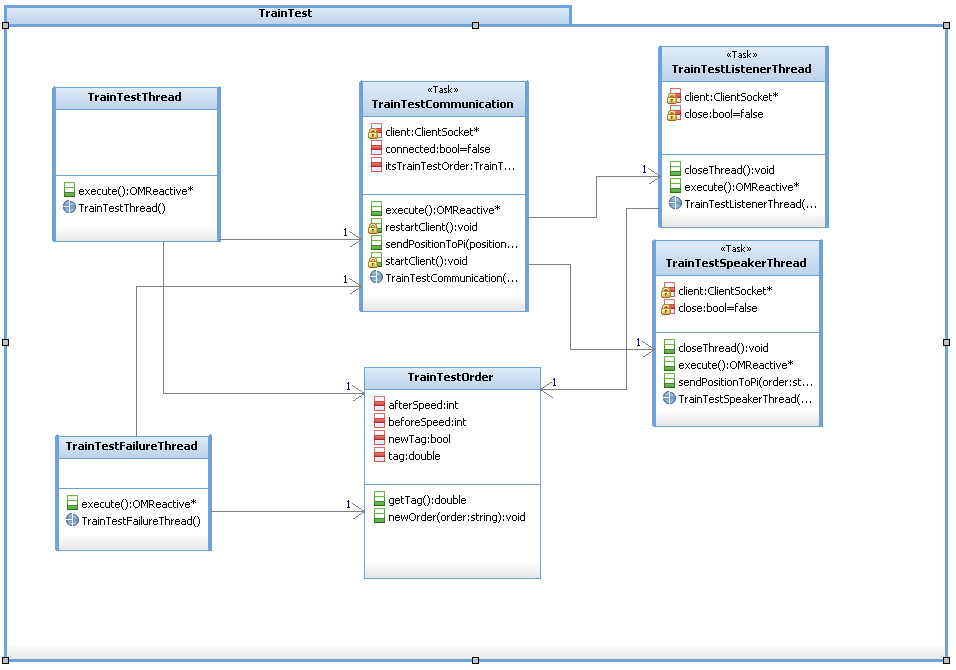
\includegraphics[width=1\textwidth]{content/pictures/train_test/train_test.png}
	\label{pic:train_test}
\end{figure}

\subsection{Testdurchführung}

Die Testdurchführung erfolgte gegen Ende des Projektes um die korrekte Ausführung des Algorithmus auch ohne Hilfe der Zughardware zu gewährleisten. Dazu wurden Algorithmus und TrainTest auf zwei unterschiedlichen Rechnern gestartet und der Ablauf anhand von Ausgaben auf der Konsole verfolgt.\\
Auch konnte die Testklasse bei Ausfällen des Zuges benutzt werden um eine Weiterentwicklung zu ermöglichen.

\section{Socket}

Zum Testen der 